\documentclass[a4paper,12pt]{extarticle}
\usepackage[utf8]{inputenc}
\usepackage{graphicx}
\usepackage{tabularx}
\usepackage{array}
\usepackage{listings}
\graphicspath{ {imgs/} }
\usepackage[margin=2cm]{geometry}
\usepackage{float}
\usepackage[thinlines]{easytable}

\setlength{\columnsep}{2em}

\lstset{basicstyle=\small\ttfamily}

\newenvironment{mono}{\fontfamily{pcr}\selectfont}{\par}

\newcommand{\image}[2] {
  % \vspace{5pt}
  % \hline
  % \vspace{5pt}
  \noindent\begin{minipage}[c]{.6\textwidth}% adapt widths of minipages to your needs
    \centering
    \strut\vspace*{-\baselineskip}\newline\includegraphics[scale=.3]{#1}
  \end{minipage}%
  \hfill%
  \begin{minipage}[c]{.4\textwidth}
    #2
  \end{minipage}
}



\title{\textbf{GIT Department Of Computer Engineering\\ 
CSE 222/505 - Spring 2020\\
Homework 8 Part 1 \vspace{1in}}}

\author{\textbf{Fatih Kaan Salgır} \\ 
\textbf{171044009}}

\date{}

\begin{document}

  \maketitle

  \newpage
  
  \section{Adjacency List Representation}
  \subsection{First Graph}

	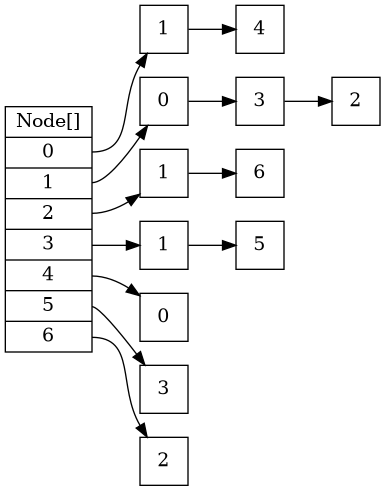
\includegraphics[scale=.4]{adjacency-list/1}

  \subsection{Second Graph}

	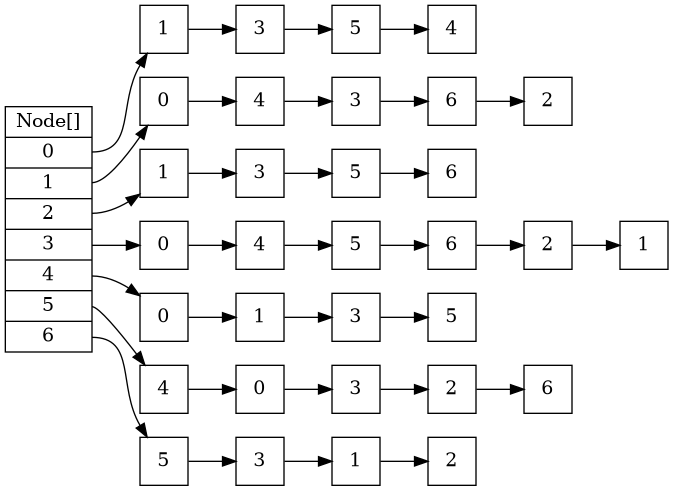
\includegraphics[scale=.4]{adjacency-list/2}

	\section{Adjacency Matrix Representation}

  \subsection{First Graph}

	\begin{mono}
		\begin{TAB}(r,1cm,1cm)[5pt]{|c|c|c|c|c|c|c|c|}{|c|c|c|c|c|c|c|c|}
		\hline
			& [0] & [1] & [2] & [3] & [4] & [5] & [6] \\
		[0] & 0 & 1 & 0 & 1 & 1 & 1 & 0 \\
		[1] & 1 & 0 & 1 & 1 & 1 & 0 & 1 \\
		[2] & 0 & 1 & 0 & 1 & 0 & 1 & 1 \\
		[3] & 1 & 1 & 1 & 0 & 1 & 1 & 1 \\
		[4] & 1 & 1 & 0 & 1 & 0 & 1 & 0 \\
		[5] & 1 & 0 & 1 & 1 & 1 & 0 & 1 \\
		[6] & 0 & 1 & 1 & 1 & 0 & 1 & 0 \\
	\end{TAB}

	\end{mono}

  \subsection{Second Graph}

	\begin{mono}
		\begin{TAB}(r,1cm,1cm)[5pt]{|c|c|c|c|c|c|c|c|}{|c|c|c|c|c|c|c|c|}
		\hline
			& [0] & [1] & [2] & [3] & [4] & [5] & [6] \\
		[0] & 0 & 1 & 0 & 0 & 1 & 0 & 0 \\
		[1] & 1 & 0 & 1 & 1 & 0 & 0 & 0 \\ [2] & 0 & 1 & 0 & 0 & 0 & 0 & 1 \\
		[3] & 0 & 1 & 0 & 0 & 0 & 1 & 0 \\
		[4] & 1 & 0 & 0 & 0 & 0 & 0 & 0 \\
		[5] & 0 & 0 & 0 & 1 & 0 & 0 & 0 \\
		[6] & 0 & 0 & 1 & 0 & 0 & 0 & 0 \\
	\end{TAB}
	\end{mono}

	\vspace{1em}

	\newpage

	\section{}

	Density is the ratio of the number of edges with respect to the maximum possible edges. Since both graphs are undirected, densitiy is; 
	$$D = \frac{2|E|}{|V|(|V|-1)}$$

	\subsection{First Graph}

	\begin{itemize}
		\item $|V| = 7$
		\item $|E| = 16$
		\item $D = \frac{2\times16}{7\times6} = 0.76$
	\end{itemize}

	\subsection{Second Graph}

	\begin{itemize}
		\item $|V| = 7$
		\item $|E| = 6$
		\item $D = \frac{2\times6}{7\times6} = 0.29$
	\end{itemize}

	To compare the representations we can consider \textbf{time efficiency} and \textbf{storage efficiency}. With respect to time efficiency, first graph is relatively dense, therefore adjacency matrix representation is better. Because even though examining all edges requires $O(V^2)$, checking if ($u, v$) is an edge requires constant time. Similarly, since second graph is sparse, list representation is better. Although checking if ($u, v$) is an edge requires $O(E_u)$, complexitiy of examining all nodes is $O(E)$.

	If we consider storage efficiency; in list representation we need to store the next cell address beside it's value. In matrix representation regardless of the number of edges, we create matrix for all possible edges. Therefore using matrix representation for dense graphs, similarly using list representation for sparse graphs is more efficient in terms of storage.

	\section{DFS Tree}

	\subsection{First Graph}

	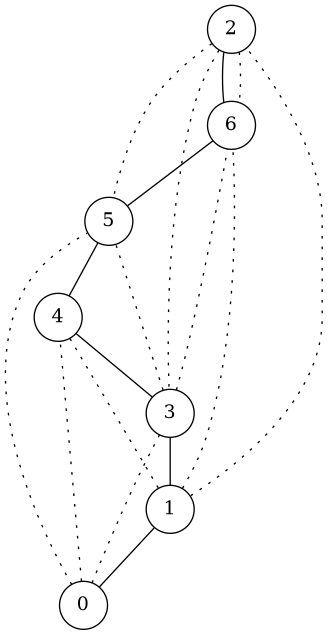
\includegraphics[scale=.6]{dfs/1}

	\subsection{Second Graph}

	\includegraphics[scale=.6]{dfs/2}

	\newpage

	\section{BFS Tree}

	\subsection{First Graph}

	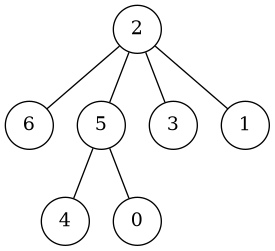
\includegraphics[scale=.6]{bfs/1}

	\subsection{Second Graph}

	\includegraphics[scale=.6]{bfs/2}


  % \image{avl/add/0.png}{Adding first node}
  % \vspace{1em}

  % \image{avl/add/1.png}{30 is greater than 20, add to right}
  % \image{avl/add/2.png}{8 is less than 20, add to left}



\end{document}
